\chapter{Analiza rozwiązań do automatycznej diagnostyki choroby Parkinsona}\label{ch:analiza-rozwiazan}


Diagnoza PD jest powszechnie oparta na obserwacjach lekarskich i ocenie objawów klinicznych, w tym charakterystyce różnorodnych objawów ruchowych.
Rosnąca liczba zachorowań i obniżenie wieku osób będących w grupie ryzyka skutkuje wzrostem zainteresowania dotyczącym narzędzi, które ułatwiłyby
zarówno codzienne funkcjonowanie pacjentów, jak i pracę lekarzy.
Tradycyjne metody diagnostyczne mogą być obarczone subiektywizmem, ponieważ opierają się między innymi na ocenie ruchów, które są czasami subtelne dla
ludzkiego oka i dlatego trudne do sklasyfikowania, co może przyczynić się do błędnej diagnozy.
Ponadto wczesne objawy niemotoryczne PD mogą być łagodne oraz spowodowane wieloma innymi schorzeniami.
Dlatego też rozpoznanie tej choroby na wczesnym etapie stanowi wyzwanie.

Sztuczna inteligencja oraz nowoczesne technologie coraz częściej stają się integralną częścią systemu ochrony zdrowia.
Wspierają lekarzy podczas diagnozy oraz wyboru sposobu leczenia pacjenta, a także pozwalają na monitorowanie choroby.
Aby rozwiązać trudności i udoskonalić procedury diagnozowania oraz oceny PD, poszerzono stan techniki o metody uczenia maszynowego do
klasyfikacji PD i osób zdrowych lub pacjentów z podobnymi objawami klinicznymi (np.
zaburzeniami ruchu lub innymi zespołami parkinsonowskimi).
\section{Rodzaj wykorzystywanych danych}\label{sec:dane-przeglad}

Diagnozowanie choroby Parkinsona stanowi zadanie złożone ze względu na różnorodność objawów, które dotykają różnych aspektów
funkcjonowania ciała i umysłu ludzkiego.
W związku z tym, techniki uczenia maszynowego wykorzystywane w tym obszarze, także skupiają się na różnych rodzajach danych.
Wśród źródeł informacji diagnostycznej znajdują się wyniki badań obrazowych (np.
rezonans magnetyczny (MRI), tomografia komputerowa (SPECT)),
które wydają się intuicyjne, biorąc pod uwagę zmiany w aktywności mózgu, które można zaobserwować.
Niemniej jednak istnieją także mniej oczywiste metody diagnozy, które budzą duże zainteresowanie w środowisku naukowym, szczególnie w początkowym stadium choroby.
Przykłady to analiza głosu, ocena charakterystyki chodu oraz badanie pisma odręcznego.

\begin{figure}[htbp]
	\centering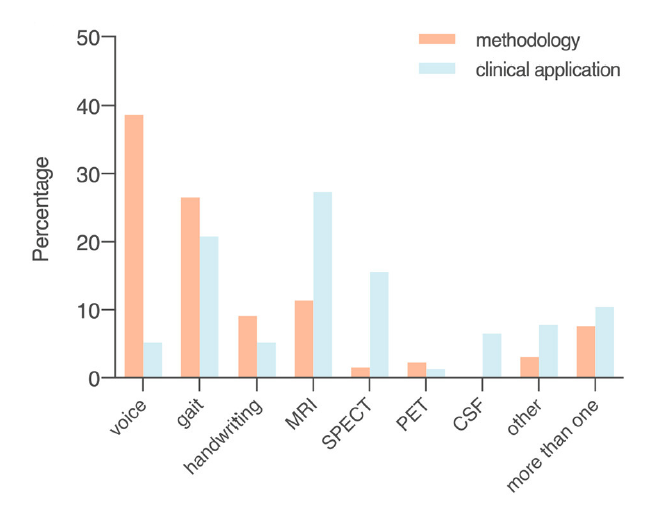
\includegraphics[width=0.6\textwidth]{./img/plot_PD_detection_methods}~\caption{Wykorzystanie rozwiązań w opracowaniach teoretycznych i zastosowaniach klinicznych w zależności od rodzaju danych (stan na 14 lutego 2020) \cite {ML_for_PD_review} }
    \label{fig:pd_detection_methods}
\end{figure}


Rys. \ref{fig:pd_detection_methods} ilustruje zastosowanie wymienionych metod zarówno w teorii, jak i praktyce.
Metody oparte na obrazowaniu medycznym wykazują wyraźną przewagę w zastosowaniach klinicznych w porównaniu do kontekstu teoretycznego.
Niemniej jednak to pozostałe metody budzą znacznie większe zainteresowanie ze strony środowiska naukowego.
Szczególnie w przypadku analizy głosu, gdzie rozbieżność między teorią a praktyką jest szczególnie znacząca.
Przyczyny tego zjawiska zostaną dokładniej rozważone w dalszej części pracy.
Co ciekawe, jak przedstawiono na Rys.~\ref{fig:pd_accuracy_methods}, detekcja choroby na podstawie głosu daje bardzo wysokie wyniki,
w większości analizowanych artykułów.

\begin{figure}[htbp]
	\centering
	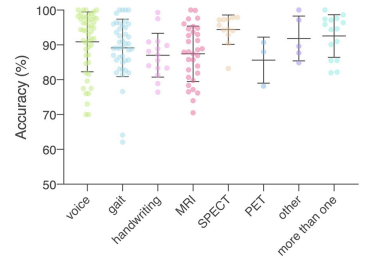
\includegraphics[width=0.6\textwidth]{./img/accuracy}~\caption{Dokładność rozwiązań diagnostycznych w zależności od rodzaju danych (stan na 14 lutego 2020) \cite {ML_for_PD_review} }
    \label{fig:pd_accuracy_methods}
\end{figure}

Niniejsza praca dotyczy diagnostyki opartej na analizie głosu, dlatego temat ten zostanie bliżej rozważony.
Założeniem dla takich systemów jest zadanie potencjalnemu pacjentowi zadania wokalnego, mogą to być:
\begin{itemize}[itemsep=0.1pt]
	\item podtrzymywane samogłoski (ang. \emph{sustained vowels}),
	\item zadanie diadochokinetyczne (DDK), mogące mierzyć zdolność do wydawania serii szybkich i naprzemiennych dźwięków (sylab),
	\item czytanie tekstu,
	\item wypowiedzenie pojedynczego zdania,
	\item monolog.
\end{itemize}

Dotychczas nie przeprowadzono badań porównawczych dotyczących wpływu wyboru zadania wokalnego na efektywność klasyfikacji w przypadku choroby Parkinsona (PD).
Jedynie w artykule~\cite{vocal_task_comparision} przeprowadzono takie porównanie, przy użyciu cech prozodii (brzmieniowych
właściwości mowy nakładających się na głoskowy, sylabiczny i wyrazowy ciąg wypowiedzi).
Nie pozwala to jednak na wyciągnięcie obiektywnych wniosków, ponieważ każde z zadań wokalnych może wymagać innego podejścia i metod klasyfikacji.
Niemniej jednak, autorzy publikacji~\cite{monitoring_speech} przeprowadzili badanie na 200 pacjentach z PD,
gdzie dokonano klasyfikacji deficytów mowy na pięć poziomów nasilenia.
Oceniono typ (głos, artykulacja, płynność) oraz zakres upośledzenia dla każdego poziomu, korzystając z 2-minutowego fragmentu mowy.
Wyniki ukazały, że głos stanowił najczęściej występujący i bardziej nasilony deficyt we wczesnych stadiach choroby.
Deficyty artykulacji i płynności pojawiały się później.
Wykazano, że upośledzenie artykulacji korelowało z upośledzeniem głosu w fazie \emph{ciężkiej}, a w fazie \emph{głębokiej} dominującą cechą była upośledzona artykulacja.

W rezultacie, w kontekście wczesnej diagnostyki choroby, artykulacja i płynność mowy nie wymagają głębokiej uwagi.
Koncentrację należy skupić przede wszystkim na cechach głosowych, co sprawia, że wybór podtrzymywanych samogłosek jako zadania wokalnego
wydaje się najlepszym wyborem ze względu na ich stabilność w czasie oraz łatwość wypowiadania przez pacjenta.
To podejście może posiadać potencjał uniwersalności dla różnych języków, co oznacza, że analiza może być stosowana
niezależnie od języka ojczystego pacjenta.
W efekcie pozwala to na bardziej efektywne i znormalizowane diagnozowanie choroby Parkinsona.

Najczęściej występującymi w opracowaniach samogłoskami są /a/, /e/, /i/ oraz /u/.
Aktualnie brakuje albo nie udało się jeszcze ustalić, która z tych samogłosek niesie najcenniejsze informacje z punktu widzenia diagnostycznego.
W związku z tym, w ramach badawczej części niniejszej pracy przeprowadzone zostanie takie porównanie dla wybranych metod klasyfikacji.
%---------------------------------------------------------------------------

\section{Metody klasyfikacji}\label{sec:metody-klasyfikacji}

W obszarze automatycznej diagnostyki choroby Parkinsona (PD) opartej na analizie głosu, istnieje wiele różnych metod klasyfikacji.
W publikacji~\cite{ML_for_PD_review} przeanalizowano 55 artykułów dotyczących tego zagadnienia, które zostały opublikowane przed lutym 2020 roku.
Analiza ujawniła, że średnia dokładność osiągnięta w tych badaniach wyniosła 90,9\%, z zakresem wyników od 70,0\%
\cite{7378178, multimodel-framework} do 100,0\% \cite{new-hybrid, fuzzy-neural-system, linear-discriminant-analysis, dastjerd}.
Wyniki były zależne od różnorodnych zbiorów danych oraz różnych podejść do analizy głosu.

Istnieje wiele czynników, które wpływają na wybór konkretnej metody klasyfikacji w zależności od kontekstu diagnostycznego.
Przykładowo, różne metody mogą być skuteczniejsze w analizie mowy spontanicznej w porównaniu do mowy kontrolowanej.
W niniejszej pracy skupiono się na metodach związanych z analizą podtrzymywanych samogłosek, co
stanowi główny obszar badawczy.

Tradycyjna inżynieria cech to jedno z najpowszechniejszych podejść w automatycznej diagnostyce choroby Parkinsona na podstawie analizy głosu.
To podejście polega na wydobyciu charakterystycznych cech z sygnału mowy, takich jak formanty, nieregularność odstępów czasowych (\emph{jitter}),
współczynniki cepstralne MFCC, stosunek poziomu hałasu do poziomu harmonicznych składników (NHR), stosunek poziomu harmonicznych składników
do poziomu szumu (HNR), wskaźnik migotania \emph{Shimmer}, częstotliwość podstawowa (F0) i wiele innych.
Choć to podejście jest popularne, istnieją również bardziej zaawansowane metody, które mogą dostarczyć dokładniejszych wyników.
Niemniej jednak tradycyjna inżynieria cech ma swoje zalety, takie jak możliwość interpretacji wyników przy użyciu powszechnie znanych miar akustycznych.

Inną perspektywą jest wykorzystanie spektrogramów jako podstawy dla procesu klasyfikacji.
Proces ten polega na przekształceniu dźwięków mowy na formę wizualną na przykład w postaci spektrogramów, które obrazują zmiany w czasie i częstotliwości.
Następnie, sieci konwolucyjne (CNN), które są zaprojektowane do pracy z obrazami, mogą analizować struktury i wzorce w spektrogramach.
To podejście może umożliwić dokładniejszą klasyfikację, szczególnie dla cech trudnych do wykrycia za pomocą innych metod.

W publikacji~\cite{Majda-Zdancewicz_Potulska-Chromik_Jakubowski_Nojszewska_Kostera-Pruszczyk} przeprowadzono porównanie tradycyjnego podejścia
opartego na inżynierii cech z nowoczesnym wykorzystaniem głębokich sieci neuronowych.
Wyniki sugerują, że połączenie tych podejść może przynieść skuteczniejsze wyniki.
Chociaż tradycyjna inżynieria cech osiągała lepsze wyniki, głębokie sieci, takie jak te z rodzin VGG i ResNet, mają potencjał do osiągnięcia jeszcze
lepszych rezultatów.

Publikacji na temat wykorzystania spektrogramów oraz CNN w klasyfikacji PD na podstawie mowy jest znacznie mniej niż tych dotyczących tradycyjnej inżynierii cech.
Spośród 55 artykułów analizowanych w~\cite{ML_for_PD_review} tylko jeden dotyczył takiego podejścia.
Jest to publikacja z 2019 roku opisana w~\cite{Gunduz}.
Badanie wprowadziło głębokie sieci neuronowe typu CNN do klasyfikacji choroby Parkinsona na podstawie cech głosowych.
Stworzono dwie struktury sieciowe, różniące się w sposobie przetwarzania cech.
Pierwsza struktura łączyła różne zestawy cech przed ich analizą w 9-warstwowej sieci CNN. Druga struktura wykorzystywała
równoległe wejścia, by jednocześnie ekstrahować głębokie cechy z różnych zestawów cech.
Wyniki wykazały, że cechy TQWT (ang. \emph{Time–Frequency Warping Transform}, rodzaj cech używanych do analizy dźwięków,
uwzględniających ich zmienne tempo w czasie i częstotliwości) były najbardziej skuteczne w klasyfikacji.
Połączenie ich z innymi cechami poprawiło wyniki.
Model drugiej struktury osiągał lepsze rezultaty niż SVM, zwłaszcza z łączeniem 3 zestawów cech.
Zaproponowane podejście CNN osiągnęło skuteczność 86,9\%, przewyższając inne metody.
Są to pierwsze obiecujące rezultaty podejścia opartego na głębokich sieciach neuronowych.

Od tamtego czasu ukazało się kilka dodatkowych publikacji, które pogłębiły ten temat.
Na przykład w publikacji~\cite{Wodzinski} zaprezentowano podejście do detekcji choroby Parkinsona, wykorzystując samogłoski o długotrwałej artykulacji oraz architekturę ResNet,
pierwotnie dedykowaną do klasyfikacji obrazów.
Obliczono spektrogramy nagrań dźwiękowych i wykorzystano je jako dane wejściowe do architektury ResNet wytrenowanej wcześniej na bazach danych ImageNet i SVD.
Osiągnięta dokładność przekraczała 90\% na zestawie walidacyjnym (PC-GITA, czyli baza danych zawierająca nagrania samogłosek od
osób posługujących się kolumbijską odmianą języka hiszpańskiego).
Wyniki pokazały, że cechy  nauczone na naturalnych obrazach potrafią przenieść wiedzę na obrazy reprezentujące spektrogram sygnału głosowego.
Co więcej, pokazano, że możliwa jest skuteczna detekcja choroby Parkinsona, wykorzystując tylko cechy oparte na częstotliwościach.


Podejście to zostało zbadane również w artykule~\cite{KARAMAN2021115013}, gdzie  porównano różne architektury CNN do automatycznej identyfikacji PD na podstawie mel-spektrogramów opierając się na uczeniu transferowym.
Porównano architektury SqueezeNet1\_1, ResNet101 i DenseNet161.
Wyniki wykazały, że zaproponowany model oparty na uczeniu transferowym z podejściem fine-tuning zapewnia akceptowalną detekcję PD z dokładnością wynoszącą 89,75\%.


Później, w 2022 roku autorzy artykułu~\cite{HIRES2022105021} wykorzystali spektrogramy oraz metodę wielokrotnego dopasowywania modelu.
Model był wstępnie trenowany na zbiorze ImageNet, następnie adaptowany do pośredniego zbioru, a na koniec dostosowywany do danych PC-GITA.
Mimo niewielkich różnic pomiędzy różnymi samogłoskami najlepszą skuteczność osiągnięto przy uwzględnieniu samogłoski /a/ uzyskując 99\% dokładności.
Co ciekawe, wykazano, że skuteczność podejścia nie zależy od płci.
To pokazuje, że metoda ma potencjał do zastosowania w praktyce klinicznej do przesiewowego badania, diagnozowania i monitorowania choroby Parkinsona.

Ciekawą analizę, również opartą na spektrogramach, opisano w publikacji~\cite{8999815}.
Zaproponowano trzy podejścia - pierwsze, wykorzystujące transfer learning; drugie, wykorzystujące głębokie cechy wyodrębnione ze
spektrogramów mowy za pomocą klasyfikatorów uczenia maszynowego; oraz trzecie, oceniające
proste cechy akustyczne nagrań również przy użyciu klasyfikatorów uczenia maszynowego.
Wyniki wskazują, że druga propozycja wykazuje obiecujące rezultaty.
Zaobserwowano najwyższą dokładność na poziomie 99,7\% dla samogłoski /o/ oraz odczytywanego tekstu przy użyciu perceptronu wielowarstwowego.
Natomiast przy wykorzystaniu głębokich cech samogłoski /i/ uzyskano dokładność wynoszącą 99,1\% przy użyciu lasu losowego.
Z badania można wywnioskować, że metoda bazująca na głębokich cechach wykazuje lepsze wyniki w porównaniu do prostych cech akustycznych i
podejść opartych na transfer learning.

Oprócz konwolucyjnych sieci neuronowych, w analizie spektrogramów wykorzystuje się również ELM (ang. \emph{Extreme Learning Machines}).
ELM to technika uczenia się maszynowego, w której warstwa wejściowa modelu jest inicjalizowana losowo, a wagi warstwy wyjściowej są wyznaczane
poprzez rozwiązanie jednokrotnego równania liniowego.
ELM ma zalety efektywności obliczeniowej oraz zdolności do radzenia sobie z różnymi typami danych,
w tym danymi wizualnymi i dźwiękowymi.
W badaniu~\cite{GUATELLI2023106700} porównano ELM oraz CNN\@.
Otrzymane wyniki mieściły się między 81,74\% a 83,91\% dokładności,
Analiza pokazała, że większa liczba próbek wpływa na lepsze wyniki, a sieć AlexNet miała najlepszą równowagę między rozproszeniem a wydajnością.
W innym badaniu~\cite{Gelvez-Almeida_2022} przeanalizowano różne wersje ELM w celu klasyfikacji pacjentów z chorobą Parkinsona.
Wyniki wskazują, że wielowarstwowe sieci ELM wykazują lepszą wydajność niż jednowarstwowe.
Osiągnięto dokładność, oscylującą w okolicach 80\%.

Sieci CNN używają metod konwolucyjnych do analizy relacji między funkcjami.
W przeciwieństwie do sieci rekurencyjnych sieci te są zazwyczaj stosowane do klasyfikacji obrazów i nie uwzględniają relacji sekwencyjnych.
Dlatego w publikacji~\cite{ER2021103006} zastosowano podejście, gdzie wyodrębnione cechy z sieci CNN są przekazywane do warstwy LSTM, aby nauczyć się
informacji czasowych w dźwiękach, rozpoznawać sekwencyjne informacje i analizować stan choroby Parkinsona.
Wykorzystano połączenie modeli ResNet LSTM\@.
Modele ResNet służą do wyciągania cech z obrazów mel-spektrogramu sygnałów mowy, a
sieć LSTM jest wykorzystywana do rozpoznawania informacji sekwencyjnych z uzyskanych cech.
Najwyższą wydajność klasyfikacji osiągnięto na poziomie 98,61\%.
Porównanie zaproponowanego modelu z aktualnym stanem wiedzy pokazuje jego wysoką wydajność w detekcji choroby Parkinsona.

Problemem, który często uniemożliwia uzyskanie zadowalających rezultatów, jest ograniczony rozmiar zbioru danych.
Większość publicznie dostępnych baz danych składa się z około 50 nagrań, co jest niewystarczające do uzyskania wiarygodnych wyników i
realnego zastosowania w medycynie klinicznej.
Specyfika choroby utrudnia też samodzielne rozszerzenie bazy o nagrania pacjentów z chorobą Parkinsona.
To wyzwanie stawiane jest przed każdym, kto próbuje stworzyć automatyczne narzędzie do diagnozowania choroby Parkinsona na podstawie analizy głosu.
W artykule~\cite{9257451} przedstawiono wykorzystanie \emph{Spectrogram-Deep Convolutional Generative Adversarial Network} (S-DCGAN) do
augmentacji próbek głosowych, co może częściowo rozwiązać próblem i przyczynić się do większej różnorodności w zbiorach danych.
Na zestawie danych Sakar, hybrydowy model S-DCGAN-ResNet50 osiągnął najwyższą dokładność rozpoznawania wzorca głosowego wynoszącą 91,25\%
oraz swoistość na poziomie 92,5\%, co pozwala na precyzyjniejsze różnicowanie między pacjentami z PD a zdrowymi osobami w porównaniu z modelem
DCGAN-ResNet50.

Wszystkie te badania prowadzą do wniosku, że wykorzystanie uczenia maszynowego oraz głębokich sieci neuronowych może istotnie poprawić precyzję
i skuteczność diagnostyki choroby Parkinsona na podstawie analizy cech głosowych.
Te nowoczesne techniki otwierają nowe horyzonty w kwestii doskonalenia opieki nad pacjentami oraz procesów diagnostycznych w dziedzinie medycyny.
Jednakże warto zaznaczyć, że wyniki te są osiągane na różnorodnych zbiorach danych, co utrudnia bezpośrednie porównania między poszczególnymi badaniami.

Najlepsze wyniki skuteczności klasyfikacji osiągnięto przy użyciu różnych podejść i modeli.
Przykładem jest metoda opisana przez Gómeza et al.~\cite{8999815}, która osiągnęła dokładność 99,7\% dla jednej samogłoski.
Z drugiej strony, istnieją też przypadki, jak w badaniu Guatelliego et al.~\cite{GUATELLI2023106700}, gdzie osiągnięto wyniki między
81,74\% a 83,91\% dokładności klasyfikacji, co może być związane z ograniczonym zbiorem danych.
Konieczne jest dalsze prowadzenie prac w tym kierunku, najlepiej na jak najbardziej rozbudowanych bazach danych.

Wartością dodaną tych badań jest możliwość zastosowania analizy głosowej w procesie diagnozowania choroby Parkinsona, co może umożliwić
wczesne wykrycie objawów i rozpoczęcie leczenia.
Wyniki te sugerują, że głębokie sieci neuronowe mogą pomóc w identyfikowaniu subtelnych cech
głosowych, które są trudne do wykrycia przez konwencjonalne metody diagnostyczne.
%---------------------------------------------------------------------------

\section{Wyzwania związane z systemami automatycznej diagnostyki}\label{sec:wyzwania}

Zainteresowanie systemami do automatycznej diagnostyki choroby Parkinsona na podstawie głosu jest ogromne i wiąże się z nim duże nadzieje.
Istnieje jednak duża dysproporcja pomiędzy pracą badawczą a ich wykorzystaniem w rzeczywistym środowisku (Rys.~\ref{fig:pd_detection_methods}).
Przyczyn takiego stanu rzeczy jest wiele, a większość z nich związana jest z brakiem usystematyzowanego podejścia do problemu, co utrudnia porównanie
rozwiązań, a tym samym rzetelny postęp.

Ostatnie badania wykazały, że możemy wytrenować dokładne modele do wykrywania oznak PD z nagrań audio.
Jednakże istnieją rozbieżności, które są częściowo powodowane przez różnice w
wykorzystywanych korpusach lub metodologii.
Dlatego autorzy publikacji~\cite{SustainedVowelsProblems} przeprowadzili analizę, wpływu niektórych czynników na wyniki klasyfikacji.
Głównym celem była ich identyfikacja oraz stworzenie zasad, które w przyszłości pozwolą usystematyzować stan wiedzy w tej dziedzinie.
W badaniach skupiono się na przedłużonych samogłoskach (ang. \emph{sustained vowels}), ponieważ są one najlepszym i najpopularniejszym zadaniem
wokalnym w takich systemach.
Przeprowadzone eksperymenty wykazały, że nieuwzględnione zmienne w metodologii, projekcie eksperymentalnym i
przygotowaniu danych prowadzą do zbyt optymistycznych wyników w badaniach nad automatyczną detekcją PD\@.
Czynniki, które zidentyfikowano jako przyczyniające się do zbyt optymistycznych wyników klasyfikacji, przedstawiono na Rys.~\ref{fig:factors_PD_detection} oraz omówiono poniżej.


\begin{figure}[htbp]
	\centering
	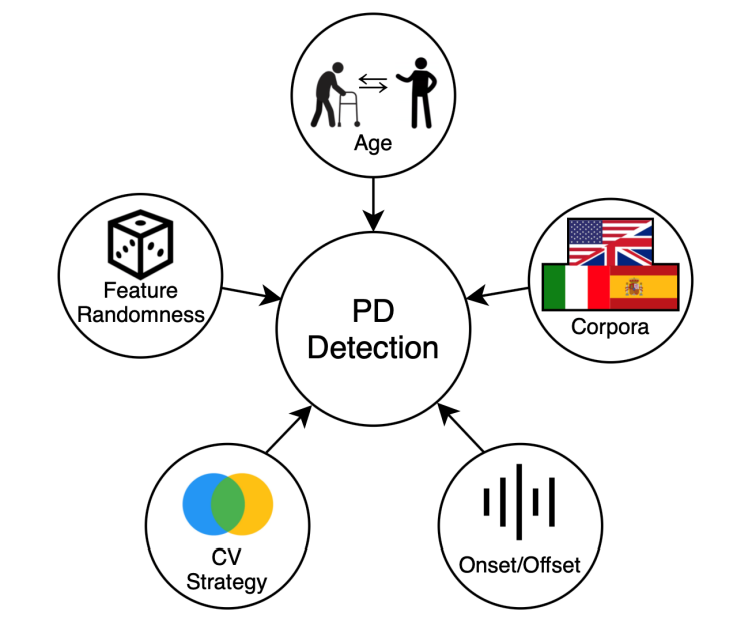
\includegraphics[width=0.4\textwidth]{./img/influence_of_factors_on_PD_detection}
	\caption{Czynniki powodujące zbyt optymistyczne wyniki detekcji PD na podstawie głosu \cite {SustainedVowelsProblems}}
    \label{fig:factors_PD_detection}
\end{figure}


\begin{enumerate}[label={\alph*)}]
	\item Pominięcie aspektu tożsamości mówcy przy konstruowaniu zbiorów treningowych i testowych
	\item[] W przypadku, gdy w zbiorze danych znajduje się kilka nagrań od tego samego mówcy, można postąpić na dwa sposoby.
Pierwszy z nich to podział według podmiotów (ang. \emph{subject-wise split}) polegający na tym, że nagrania od tej samej
osoby znajdują się albo w zbiorze treningowym, albo testowym, natomiast nigdy w obu na raz.
Drugie podejście to podział według rekordów (ang. \emph{record-wise split}), gdzie nagrania są losowo dzielone do zbiorów
lub intencjonalnie używa się nagrań od tej samej osoby zarówno w zbiorze testowym, jak i treningowym.
Okazuje się, że podejście typu \emph{record-wise} prowadzi do wyższej dokładności niż \emph{subject-wise split}, jeśli pozostałe założenia pozostają identyczne.
Prawdopodobnie wynika to z faktu, że klasyfikator nastawia się na wykrywanie unikalnych informacji indywidualnych,
reprezentowanych przez współczynniki takie jak MFCC, a nie rzeczywiste biomarkery lub wzorce PD\@.
Dlatego też rekomendowana jest technika \emph{subject-wise split}, aby uniknąć zbyt optymistycznych wyników.

  	\item Niezbalansowanie klas pod względem wieku
	\item[] W literaturze można znaleźć prace wykorzystujące zbiory danych, w których średni wiek mówców
w klasie osób chorych na PD różni się od średniego wieku w klasie osób zdrowych o ponad 5 lat.
Autorzy zapewniają o wysokiej skuteczności swoich rozwiązań, jednak pomijają informacje o ryzyku, że klasyfikator
uczy się wykrywać cechy powiązane z wiekiem, zamiast rzeczywistych wzorców PD\@.
Wyniki eksperymentów w publikacji~\cite{SustainedVowelsProblems} pokazują, że wraz ze wzrostem różnicy między średnim wiekiem uczestników z PD i HC,
dokładność klasyfikacji konsekwentnie rośnie (Rys.~\ref{fig:acc_and_age_diff}).
Na tej podstawie można stwierdzić, że związany z wiekiem wpływ na głos mówców może zaburzać wyniki otrzymywane przez klasyfikator.
Dlatego też zaleca się zbalansowanie używanych zbiorów danych, tak aby średnia różnica wieku między tymi dwoma klasami była jak najmniejsza.


\begin{figure}[htbp]
	\centering
	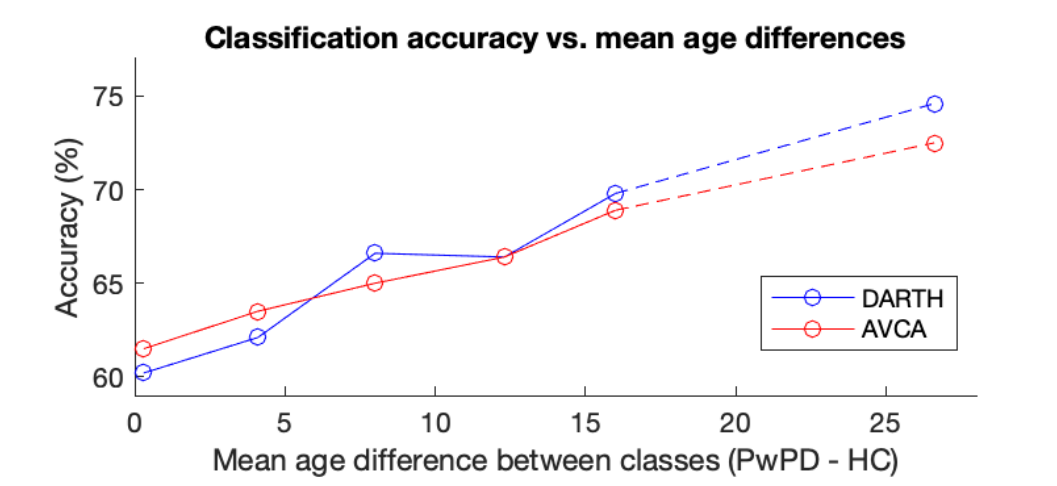
\includegraphics[width=0.7\textwidth]{./img/acc_and_age_difference}
	\caption{Wykres przedstawiający zależność różnicy wieku między klasami a dokładnością klasyfikacji~\cite {SustainedVowelsProblems}}
    \label{fig:acc_and_age_diff}
\end{figure}

  	\item wpływ losowości cech na dokładność klasyfikacji
	\item[] W publikacji~\cite{SustainedVowelsProblems} przeprowadzono badania analizujące wpływ losowości cech na dokładność klasyfikacji.
Zamieniono cechy obliczone za pomocą DARTH-VAT na losowe liczby, zachowując etykiety i podziały.
Wyniki wskazały, że nawet losowe cechy mogą prowadzić do wysokich wyników klasyfikacji (ponad 72\%).
Efekt ten jest bardziej widoczny w mniejszych korpusach, gdzie różnica między liczbą nagrań a wymiarowością cech ma większy wpływ na potencjalną korelację przypadkową.
Badanie pokazuje, że nadmierna liczba cech w stosunku do liczby obserwacji może prowadzić do fałszywie wysokich wyników klasyfikacji nawet przy użyciu losowych cech.
Im większa różnica między liczbą plików a wymiarem wektora cech, tym większe szanse na znalezienie cechy, która losowo koreluje z etykietami klas.
To sugeruje, że osiągnięcia klasyfikacyjne powinny być analizowane w kontekście proporcji cech do próbki, aby uniknąć nadmiernie optymistycznych interpretacji wyników klasyfikacji w zastosowaniach medycznych.

  	\item ograniczenie losowego nadmiernego dopasowania poprzez uwzględnienie zbioru walidacyjnego
	\item[] Dla mniejszych zbiorów danych, praktyką jest często używanie tylko zbiorów treningowych i testowych podczas krzyżowej walidacji.
Jest to podejście, które może prowadzić do wyników zbyt optymistycznych, ponieważ wszystkie wyniki testowe są brane pod uwagę przy wyborze optymalnej
konfiguracji modelu.
Inną strategią jest wykorzystanie danych treningowych do oceny wytrenowanych modeli i późniejsze przetestowanie najlepszego modelu na zbiorze testowym.
Niemniej jednak to podejście może być niepraktyczne, ponieważ może prowadzić do wyników idealnych (dokładność 100\%) na zbiorze treningowym, co jest niepożądane.
Aby uniknąć tych problemów, proponuje się wykorzystanie dodatkowego zbioru walidacyjnego~\cite{SustainedVowelsProblems}.
Wybierając model na podstawie wyników walidacyjnych, a następnie testując go na zbiorze testowym, można uniknąć ryzyka nadmiernego dopasowania.
Dla mniejszych zbiorów danych ta strategia może ograniczać dostępną liczbę danych treningowych, co wpływa na wydajność klasyfikacji.

	\item wpływ początku i końca  nagrań samogłosek na wyniki klasyfikacji
\item[] Główną różnicą między korpusami wykorzystywanymi do klasyfikacji choroby Parkinsona jest obecność fragmentów nagrania oznaczonych jako \emph{onset} i \emph{offset}.
Niektóre nagrania zawierają te segmenty, podczas gdy inne zostały ich pozbawione, aby zapewnić stabilniejszą fonację, co jest korzystne dla pewnych cech i algorytmów analizy.
W celu oceny znaczenia informacji zawartych w obszarach \emph{onset} i \emph{offset} dla klasyfikacji przeprowadzono eksperymenty porównawcze,
wykorzystując nagrania zarówno z fragmentami przyciętymi, jak i nieprzyciętymi~\cite{SustainedVowelsProblems}.
Wyniki tych eksperymentów ukazały, że wyeliminowanie fragmentów początkowych i końcowych wpłynęło negatywnie na dokładność klasyfikacji.
To wskazuje na to, że obszary te zawierają istotne informacje artykulacyjne, które mają znaczenie dla procesu klasyfikacji.

 	\item eksperymenty międzykorpusowe a zdolności generalizacyjne
	\item [] Większość badań dotyczących diagnozowania choroby Parkinsona na podstawie głosu opiera się na jednym lub ewentualnie kilku (wykorzystywanych niezależnie)
korpusach mowy.
W tym kontekście często pomija się badanie zdolności klasyfikatorów do ogólnego zastosowania.
W artykule~\cite{SustainedVowelsProblems} przeprowadzono międzykorpusowe eksperymenty na bazach danych w językach włoskim i hiszpańskim w celu
przetestowania zdolności ogólnych modeli.
Skuteczność tych modeli różniła się w zależności od języka zbioru testowego.
Może to wynikać z odmiennej różnorodności nagrań, co ma wpływ na stabilność modelu.
Drugim możliwym wyjaśnieniem jest to, że głos osób z chorobą Parkinsona może być w różnym stopniu obarczony objawami choroby w zależności od języka ojczystego lub stopnia zaawansowania choroby.
Innymi słowy, w zależności od użytego zbioru danych objawy mogą być nasilone w różny sposób i konieczne jest wzięcie tego pod uwagę tak by zdolności generalizacyjne modelu były jak najwyższe.
\end{enumerate}


Identyfikacja i świadomość wpływu powyższych czynników pozwala na dostosowaniu przeprowadzanych eksperymentów tak, aby uniknąć wyników zbyt optymistycznych.
Usystematyzowanie podejścia do analizy głosu pod kątem diagnostyki choroby Parkinsona przyczyni się do możliwości obiektywnego porównania istniejących i nowych rozwiązań.
Tym samym przyspieszy to postęp w tej dziedzinie i uzyskanie optymalnego rozwiązania, które mogłoby zostać wykorzystane w rzeczywistym środowisku.

Nie są to jednak wszystkie czynniki, które zaburzają obiektywność wyników.
Konieczna jest dyskusja na temat nowych kompleksowych linii bazowych dla prowadzenia eksperymentów w automatycznym wykrywaniu PD na podstawie fonacji,
a także innych ogólnych zastosowań przetwarzania mowy.

Prace nad automatyczną detekcją Parkinsona na podstawie głosu trwają już od dłuższego czasu.
Jednak wciąż brakuje systemu, który mógłby zostać uznany za wystarczająco niezawodne narzędzie diagnostyczne.
Wśród problemów, które ograniczają rzeczywiste wykorzystanie takich systemów wyróżnia się:
\begin{itemize}[itemsep=0.1pt]
	\item zróżnicowanie wzorców mowy: osoby z chorobą Parkinsona mogą różnić się w sposób, w jaki zmiany w mowie wpływają na ich głos.
To zróżnicowanie utrudnia stworzenie uniwersalnego modelu, który działałby skutecznie dla wszystkich pacjentów.
	\item wpływ zmiennych czynników: wpływ na mowę mogą mieć różne czynniki, takie jak zmęczenie, stres czy otoczenie akustyczne.
Te zmienne mogą wprowadzać zakłócenia w analizie mowy i utrudniać jednoznaczną diagnozę.
	\item potrzeba dużej bazy danych: aby stworzyć dokładny system detekcji, konieczne jest posiadanie dużej bazy danych głosów osób z i
bez choroby Parkinsona.
Uzyskanie takiej bazy danych, która odzwierciedla różnorodność pacjentów i warunki środowiskowe, może być wyzwaniem.
Większość publikacji opiera się na bazach danych zawierających około 50 nagrań, co nie jest wystarczająco reprezentatywną próbą.
	\item wczesne wykrycie i subtelne objawy: wczesne stadia choroby Parkinsona często manifestują się subtelnie, a różnice w mowie mogą być
trudne do zauważenia.
To może prowadzić do błędnych diagnoz lub niskiej skuteczności systemu.
	\item weryfikacja i walidacja: Aby narzędzie diagnostyczne oparte na mowie było skuteczne, musi być poddane rygorystycznym testom w rzeczywistych
warunkach klinicznych.
Weryfikacja i walidacja takiego systemu to skomplikowany proces.
	\item ograniczenia technologiczne: pomimo postępów w technologii analizy mowy, istnieją nadal ograniczenia w dokładności i precyzji takich systemów.
Może to prowadzić do wyników fałszywie pozytywnych lub negatywnych.
	\item aspekty etyczne i prywatność: wykorzystywanie danych głosowych do diagnozowania chorób podnosi kwestie związane z prywatnością i etyką.
Konieczne jest zagwarantowanie odpowiednich zabezpieczeń danych i zgody pacjentów na wykorzystanie ich informacji w celach medycznych.
\end{itemize}

Mimo tych wyzwań, prace nad wykorzystaniem analizy mowy do diagnozowania choroby Parkinsona są obiecujące i mogą przyczynić się do poprawy jakości życia
pacjentów oraz usprawnienia procesu diagnozy i leczenia.
Jednakże przed stworzeniem skutecznego narzędzia diagnostycznego opartego na głosie jest jeszcze wiele pracy do wykonania

W niniejszej pracy podjęta zostanie próba implementacji takiego rozwiązania.
Uwzględnione zostaną wszystkie z rekomendacji przedstawionych w artykule~\cite{SustainedVowelsProblems}.